\documentclass[letterpaper]{article}
\usepackage[utf8]{inputenc}
\usepackage[margin=1.25in]{geometry}
\usepackage{parskip, tikz, amsmath, hyperref, listings, pgffor, courier, color, graphicx}
\usetikzlibrary{arrows.meta, arrows}

\definecolor{mygreen}{rgb}{0,0.6,0}
\definecolor{mygray}{rgb}{0.5,0.5,0.5}
\definecolor{mymauve}{rgb}{0.58,0,0.82}

\lstset{
  basicstyle=\small\ttfamily,
  commentstyle=\color{mygreen},
  keywordstyle=\color{blue},
  stringstyle=\color{mymauve}
}

\title{Automating Data Structure Transformations Through Type Chaining}

\author{
  Martin Schneider\\
  \texttt{martinfs@mit.edu} \and
  Josh Gruenstein\\
  \texttt{jgru@mit.edu}
}

\date{6.905 Spring 2019}
 
\begin{document}
 
\maketitle

\begin{abstract}
We propose a system for automating multi-step type transformations in MIT Scheme.  After registering a set of predicates and transformations between them, the programmer can request data be transformed into a given predicate, or set of predicates.  The system then performs a backtracking search to find an appropriate type conversion flow, and can either perform the conversion or return generated conversion code.  This eliminates much of the boilerplate and mental overhead involved in many software systems dealing with data of different types.
\end{abstract}

\section{Introduction}

Much of programming involves manipulation and transformation of data into different types.  Internet connected systems serialize HTTP data into some format, then translate to a JSON type and finally to a normal data structure.  An image processing system may convert images from a filename to a JPEG type to a RGB type to a gray-scale image.  A command line program might parse a command line input, to a split list, to a data-structure with \texttt{int}s and \texttt{string}s and \texttt{flag}s, and finally to commands to be executed.

\begin{figure}[h!]
\centering

\resizebox{14cm}{!} {
  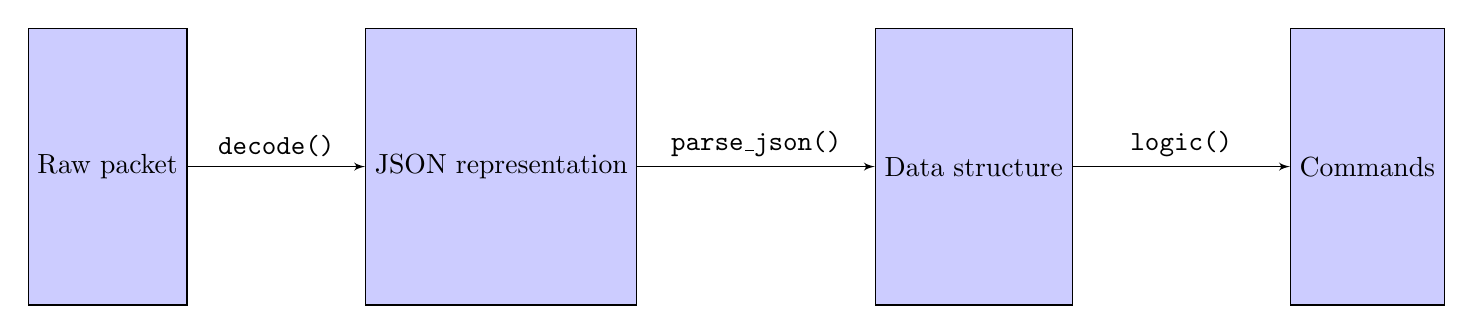
\begin{tikzpicture}[node distance=2.5cm,auto,>=latex']
	\tikzstyle{type}=[draw, fill=blue!20, minimum size=2em,minimum height=10em]
	\tikzstyle{init} = [pin edge={to-,thin,black}]

    \node [type] (a) {Raw packet};
    \node [type] (c) [right of=a, node distance=5cm] {JSON representation};
    \node [type] (d) [right of=c, node distance=6cm] {Data structure};
    \node [type] (e) [right of=d, node distance=5cm] {Commands};
    
    \path[->] (a) edge node {\texttt{decode()}} (c);
    \draw[->] (c) edge node {\texttt{parse\_json()}} (d);
    \draw[->] (d) edge node {\texttt{logic()}} (e);
\end{tikzpicture}
}

\caption{A type conversion diagram for a webserver.}
\label{webserver}
\end{figure}

Languages with type annotations or inference often have the information necessary to infer these flows, but instead force the programmer to explicitly notate the conversion process.  This leads to more code and more thinking, which we believe to be universally worse than less code and less thinking.

To remedy this, we propose a system capable of automatically generating these conversion flows.  To achieve this, we built the following functionality in MIT Scheme, which we'll elaborate on in later sections:

\begin{enumerate}
  \item A method of registering predicates: functions that match a certain type.
  \item A method of registering sub-types of predicates.
  \item Support for ``compound predicates,'' groups of element-wise predicates that match lists.
  \item A method of registering conversions between predicates, building up a ``predicate conversion graph'' where nodes represent predicates, and edges represent transformations on predicates and an accompanying transformation on data that matches the start predicate.
  \item A search engine that, given an input predicate, explores the predicate conversion graph to find paths to a given output predicate.
  \item A programmer-facing API for explicitly converting data, exploring conversion paths, and generating type conversion code.
\end{enumerate}

We'll demonstrate how this system provides an extremely flexible basis for automatic type conversion using multiple examples.

\section{Type System}

Trivially, any system capable of finding type transformations must have a type system, where the inputs and outputs of functions are labeled with a given type.  We chose to use predicates to represent our types: functions that return true if the input matches the type.  This provides us with a simple and flexible type system.  We then provide functionality to \textit{register} predicates by adding them as nodes to our predicate conversion graph, such that they can be used by the system.

\begin{figure}[h!]
\centering
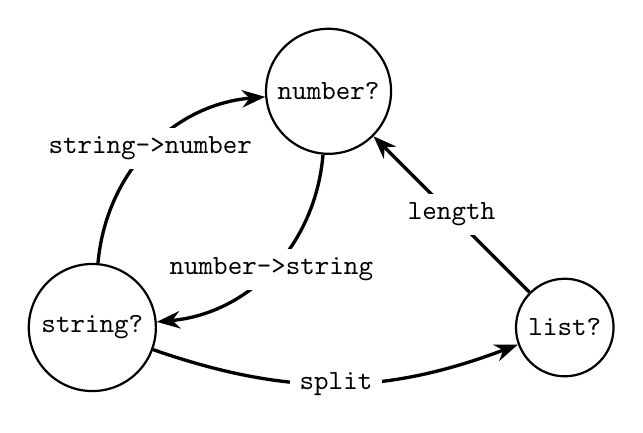
\begin{tikzpicture}
\begin{scope}[every node/.style={circle,thick,draw}]
    \node (A) at (0,0) {\texttt{string?}};
    \node (B) at (3,3) {\texttt{number?}};
    \node (C) at (6,0) {\texttt{list?}};
\end{scope}

\begin{scope}[>={Stealth[black]},
              every node/.style={fill=white},
              every edge/.style={draw=black,very thick}]
    \path [->] (A) edge[bend left=40] node {\texttt{string->number}} (B);
    \path [->] (B) edge[bend left=40] node {\texttt{number->string}} (A);
    \path [->] (C) edge node {\texttt{length}} (B);
    \path [->] (A) edge[bend right=20] node {\texttt{split}} (C);
\end{scope}
\end{tikzpicture}
\caption{An example predicate conversion graph.}
\label{graph}
\end{figure}

In this graph, edges represent transformations between predicates.  However, unlike what the figure above may suggest, our system's type conversion graph is dynamic; rather than storing edges as having a source and a sink, edges have a source and a predicate transformation function, which given the source returns a sink.  This allows fancy inferred conversions using dynamic types, such doubling lists of arbitrary lengths.

In addition to the predicate transformation graph, we also store a graph of predicate subtypes and super-types.  We chose to use a separate data structure for this (rather than just creating identity transformations in the predicate conversion graph) in order to allow using super-type transformations without losing information from the original predicate.  For example, in the list doubling example, imagine a \texttt{list-len-2?} predicate were transformed into a \texttt{list?} predicate such that it could be doubled.  Doing so would lose the information that the list is of length two, forcing the search to occur on the actual data rather than just on the predicates.  This would be far more computationally intensive and could lead to negative side effects from actually executing transformations during the search without the programmer's permission. 

\section{Search Engine}

Given the previously defined predicate conversion graph, conversion paths between simple predicates such as \texttt{string?}, \texttt{number?}, and even \texttt{list-len-2?} can be found with a basic backtracking search.  Introducing subtypes only slightly increases complexity by forcing the search to consider edges not only from the source node, but also from any supertype nodes.

However, if we want to allow even more complex type chaining, we should be able to operate not just on predicates, but on groups of predicates, or ``compound predicates''.  For example, if we define a transformation from \texttt{(number? number?)} to \texttt{point?}, our search engine should be able to convert \texttt{(string?, string?)} to \texttt{point?}.  We call these operations on compound predicates \textit{compound transformations}.

Finally, in addition to being able to manipulate and transform compound predicates, we should also be able to branch transformations to form them.  Using our \texttt{point?} example again, if we've defined \texttt{point:x} and \texttt{point:y} as transformations from \texttt{point?} to \texttt{number?}, we should be able to infer a path from \texttt{point?} to \texttt{(number? number?)}.  We call these operations of branching into compound predicates \textit{joiner transformations}.

Our search engine supports both compound, joiner, and normal transformations.

\subsection{Handling of compound transformations}

Our standard search process works by querying the predicate transformation graph to find all possible transformations, filtering out predicates already visited in the current type flow, then recursing to try each transformation.  We extend this to compound transformations by considering each possible transformation of each predicate (or none), and taking the crossproduct of the predicate transformations to get each possible transformation for the compound predicate.

\begin{figure}[h!]
\centering
\texttt{(string? number?)} $\rightarrow \begin{bmatrix}
  \texttt{string?} \\
  \texttt{number?} \\
  \texttt{list?}
\end{bmatrix} \times \begin{bmatrix}
  \texttt{number?} \\
  \texttt{string?}
\end{bmatrix} \rightarrow \, \begin{matrix}
  \texttt{(string? number?)} \\
  \texttt{(string? string?)} \\
  \texttt{(number? number?)} \\
  \dotsc \\
  \texttt{(list? string?)}
\end{matrix}$

\caption{Transformations of \texttt{(string? number?)} using the Figure \ref{graph} graph.}
\label{crossproduct}
\end{figure}

We can now filter out already visited transformations, and recurse on the remaining transformations to explore paths they may be a part of.

\subsection{Handling of joiner transformations}

As discussed above, we'd like to be able to branch predicates into compound predicates.  One motivating example for this is the \texttt{person?} record type, with attributes \texttt{person:first} and \texttt{person:last}, each with corresponding predicates.  We'd like to be able to automatically convert a \texttt{person?} into a \texttt{(person:first? person:last?)}.  We handle these joiner transformations the following way:

\begin{enumerate}
  \item Find all possible compound predicate targets or sub-targets by looking at the conversion target and at all compound predicates registered in the predicate conversion graph.
  \item Filter out compound predicates that cannot reach the target predicate, and find a path for those who can.
  \item Find a path from the input predicate to each predicate in each workable compound predicate.  If any predicate cannot be reached, neither can the compound predicate.
  \item Return all compound predicates that work, the paths from them to the target, and to them from the input.
\end{enumerate}

This method is less efficient than, for example, working backwards from the target predicate.  However, it is an extensible modification to the original search process, and is likely asymptotically equivalent.

\section{API Reference}

Programmers can interact with our system through the following method calls.  More complete examples can be found in our codebase, linked to in Appendix A.

\newcommand{\doc}[3]{\item \texttt{#1}: #2\\\\Example: \texttt{#3}}

\begin{list}{$>$}{}
  \doc{(register-predicate! predicate)}
  {Registers a given predicate by adding it to the predicate conversion graph.}
  {(register-predicate! number?)}

  \doc{(register-super! subpredicate superpredicate)}
  {Registers a predicate as a subpredicate of another predicate.}
  {\\(define (is-three? num) (eq? num 3))\\
  (register-super! is-three? number?)}
  
  \doc{(register-type-transform! input-type output-type transformation-function)}{Registers a function as a transformation between two registered predicates.}{(register-type-transform! number? string? number->string)}

  \doc{(register-type-transform-f! input-type predicate-transform-function \\transformation-function)}{Registers a function as a transformation from the input predicate, into a new predicate generated by a predicate transform function.  See \\\texttt{example-list-types.scm} for an example of where this could be useful.}{\\(register-type-transform! number? (lambda (x) string?) number->string)}

  \doc{(get-transformations input-predicate output-predicate)}{Returns a list of transformations from the input predicate to the output predicate.}{(get-transformations string? number?)}

  \doc{(create-compound-transformation transformation-path)}{Given a transformation path from \texttt{get-transformations}, return a method that transforms according to that path.}{\\((create-compound-transformation (car\\
  (get-transformations number? string?))) 5)}

  \doc{(transform-with-first-path input-predicate output-predicate input-value)}{Find the first path between the input and output predicates, and transform the input accordingly.}{(transform-with-first-path number? string? 5)}

  \doc{(transform-with-first-path input-predicate output-predicate input-value)}{Find the first path between the input and output predicates, and transform the input accordingly.}{(transform-with-first-path number? string? 5)}

  \doc{(debug-get-transformations-values input-predicate output-predicate input-value)}{Return a list of all possible transformations of input-value, while printing to the console the transformation paths, intermediate values, and autogenerated code.}{(debug-get-transformations-values number? string? 5)}

  \doc{(debug-transform-to input-value output-predicate)}{Infer the input type, and return all possible transformations to the output-predicate while printing path information to the console.}{(debug-transform-to 5 string?)}
\end{list}


\section{Discussion}

A common goal of programming languages is to minimize the amount of code that needs to be written.  The programmer should be able to specify what they want as tersely as possible, and the computer should do the rest.  We propose one such mechanism for allowing computers and languages to infer large components of programs, by focusing on types and conversion flows between them.  Changing one's perspective to view more of computation as type conversion provides a framework from which more of the program can be easily inferred by a smart compiler.

Another interesting aspect of this project is the collaborative nature between our system and the programmer.  By being less verbose in our programming, we force the system to ask us clarifying questions; in this case, which type flow to pick.  We think this is a necessary trade-off for more advanced programming environments, and possibly a useful direction for future research.

We'd also like to note that many of the ideas in this paper are not wholly original.  Our type inference is similar to Prolog's logic-based programming.  Scala has ``implicit conversions,'' which allows the definition of automatic conversions between types (but not chaining without significant extra work).

\appendix
\section{Github Repo Link}

All of our code (including the \LaTeX\, source for this writeup) can be found at the following link:

\begin{center}
  \url{https://github.com/mfranzs/6905-final-project}
\end{center}

We also provide a hard copy in the following pages.

\section{Source Code}

\newcommand*{\sourcefiles}{
    main,
    example-basic,
    example-compound-types,
    example-list-types,
    example-record-types,
    helpers,
    load,
    memoize%
}

\foreach \c in \sourcefiles {
  \subsection{\c.scm}
  \lstinputlisting[language=lisp]{../\c.scm}
}


\end{document}
